\section{Ways to look at it}

Reference: \href{https://youtu.be/TkwXa7Cvfr8?si=V8cJG_DQAoA2fndE}{Watching Neural Networks Learn}\\

An \gls{AI_NN} is a \textit{non-linear mathematical tool} intended to simulate the human brain process by using simple units called artificial neurons arranged in structures known as layers.
\begin{center}
	An \gls{AI_NN} is a \textit{universal function approximator}. They are machines that create functions.
\end{center}

This non-linear mathematical tool can also be understood as a \textit{universal function approximator}. The \textit{Universal Approximation Theorem} states that \gls{AI_NN} with infinite neurons can approximate any function given the right weights. How to achieve this or how to come closer should be the objective of this segment. For example, the layer architecture, the activation function, and preparing the data are relevant topics to consider for finding the global minimum.

\paragraph{Different ways to look at it}
Many mathmatical field are in interplay when it comes to a \gls{AI_NN}.\\

Linear Algebra is mostly used when it comes to computing information though the network. Graph Theory can also be used to to the same thing, but is mostly considered when it comes to analyzing the structure of the neural network. 

\begin{description}
	\item[Linear Algebra] \glspl{AI_NN} can be represented using matrices and vectors, where each neuron's input and output can be described as linear combinations of the inputs with corresponding weights. Matrix operations such as multiplication, addition, and transposition are fundamental in understanding how information flows through the network during forward and backward propagation.
	\item[Graph Theory] \glspl{AI_NN} can be represented as directed graphs, where neurons correspond to nodes and connections between neurons correspond to edges. Graph theory concepts are useful for analyzing the structure of neural networks, including connectivity patterns and network architectures.
\end{description}

Given a certain structure of the network \textit{optimisation} with main tool from \textit{calculus}: \textit{gradient descent} is used to find the parameter that reduces the loss function.\footnote{
	While calculus and optimization are related and often used together in the context of machine learning and neural networks, they are distinct mathematical concepts with different focuses.
}

\begin{description}
	\item[Optimization] \gls{AI_NN} are trained by optimizing a loss function with respect to the network's parameters. Optimization theory provides a framework for selecting appropriate optimization algorithms, tuning hyperparameters, and understanding convergence properties. While calculus provides the mathematical framework for computing gradients and understanding the behavior of optimization algorithms, optimization theory encompasses a wider range of techniques beyond calculus, such as convex optimization, linear programming, and heuristic algorithms.
	\item[Calculus (Optimization)] Calculus is essential for optimizing the parameters (weights and biases) of \gls{AI_NN} through techniques like gradient descent and its variants. Understanding derivatives is crucial for computing gradients, which indicate how the loss function changes with respect to changes in the network's parameters. Calculus helps in finding the direction and rate of change that minimizes or maximizes a function, which is crucial for training neural networks to minimize the loss function.
\end{description}

The field of \textit{probability and statistics} as well as \textit{information theory} are used for multiple aspects of \glspl{AI_NN}. For example the former can be used to preparing or preprocessing of data, model evaluation and bringing into context the uncertainty in predictions. The later will also be used for finding the features in the dataset as well as analysing the information flow inside a \gls{AI_NN}.

\begin{description}
	\item[Probability and Statistics] ANNs can be viewed as probabilistic models, especially in the context of Bayesian neural networks, where uncertainty is explicitly modeled. Statistical techniques are used for data preprocessing, model evaluation, and uncertainty estimation in predictions.
	\item[Information Theory] Information theory concepts, such as entropy and mutual information, can be used to analyze the information flow within neural networks. Compression techniques inspired by information theory, such as autoencoders, are used for feature extraction and dimensionality reduction.
\end{description}

The field of \textit{functional analysis} provides the tools to analyze the natrue of the universal function approximator, called \gls{AI_NN}.

\begin{description}
	\item[Functional Analysis] \glspl{AI_NN} can be viewed as function approximators, and functional analysis provides tools for analyzing the properties of these approximations. Understanding function spaces and convergence properties is relevant when studying the expressive power and generalization abilities of neural networks. 
\end{description}

\pagebreak

\begin{sidewaystable}[htbp] %Doesn't accept placement parameters
	\centering
	\begin{tabular}{|p{3cm}|*{6}{p{3cm}|}}
		\hline
		\textbf{Mathematical Fields} & \textbf{Featurization} & \textbf{Data Processing} & \textbf{Model Architecture} & \textbf{Optimization Parameter} & \textbf{Evaluation} & \textbf{General Assessment} \\ \hline
		\textbf{Linear Algebra} & ~ & ~ & ANN represented as matrices and vectors; Input and Output linear combination & ~ & ~ & ~ \\ \hline
		\textbf{Graph Theory} & ~ & ~ & ANN represented as directed graphs; Analyzing the structure of the network & ~ & ~ & ~ \\ \hline
		\textbf{Information Theory} & Compression techniques: autoencoder; dimensionality reduction & ~ & ~ & ~ & ~ & ~ \\ \hline
		\textbf{Optimization (e.g., Calculus)} & ~ & ~ & ~ & Techniques like gradient descent and weights and biases & ~ & ~ \\ \hline
		\textbf{Probability Theory (Stochastic)} & ~ & Techniques for data processing steps & In case of a BNN & ~ & Model evaluation; uncertainty estimation in predictions & ~ \\ \hline
		\textbf{Functional Analysis} & ~ & ~ & ~ & ~ & ~ & Understanding the expressive power/general ability \\ \hline
	\end{tabular}
	\caption{Workflow Diagram of Mathematical Perspectives in ANN}
\end{sidewaystable}
\pagebreak

\paragraph{Landscape of different Architectures}

There are different kinds of \gls{AI_NN}, for example: convolutional, recursive. This segment will focus on \textit{feed-forward} networks. A Feed-Forward is usually a non-linear regression or classification with a sigmoidal activation and a multilayer perceptron.

\begin{figure}[H]
	\centering
	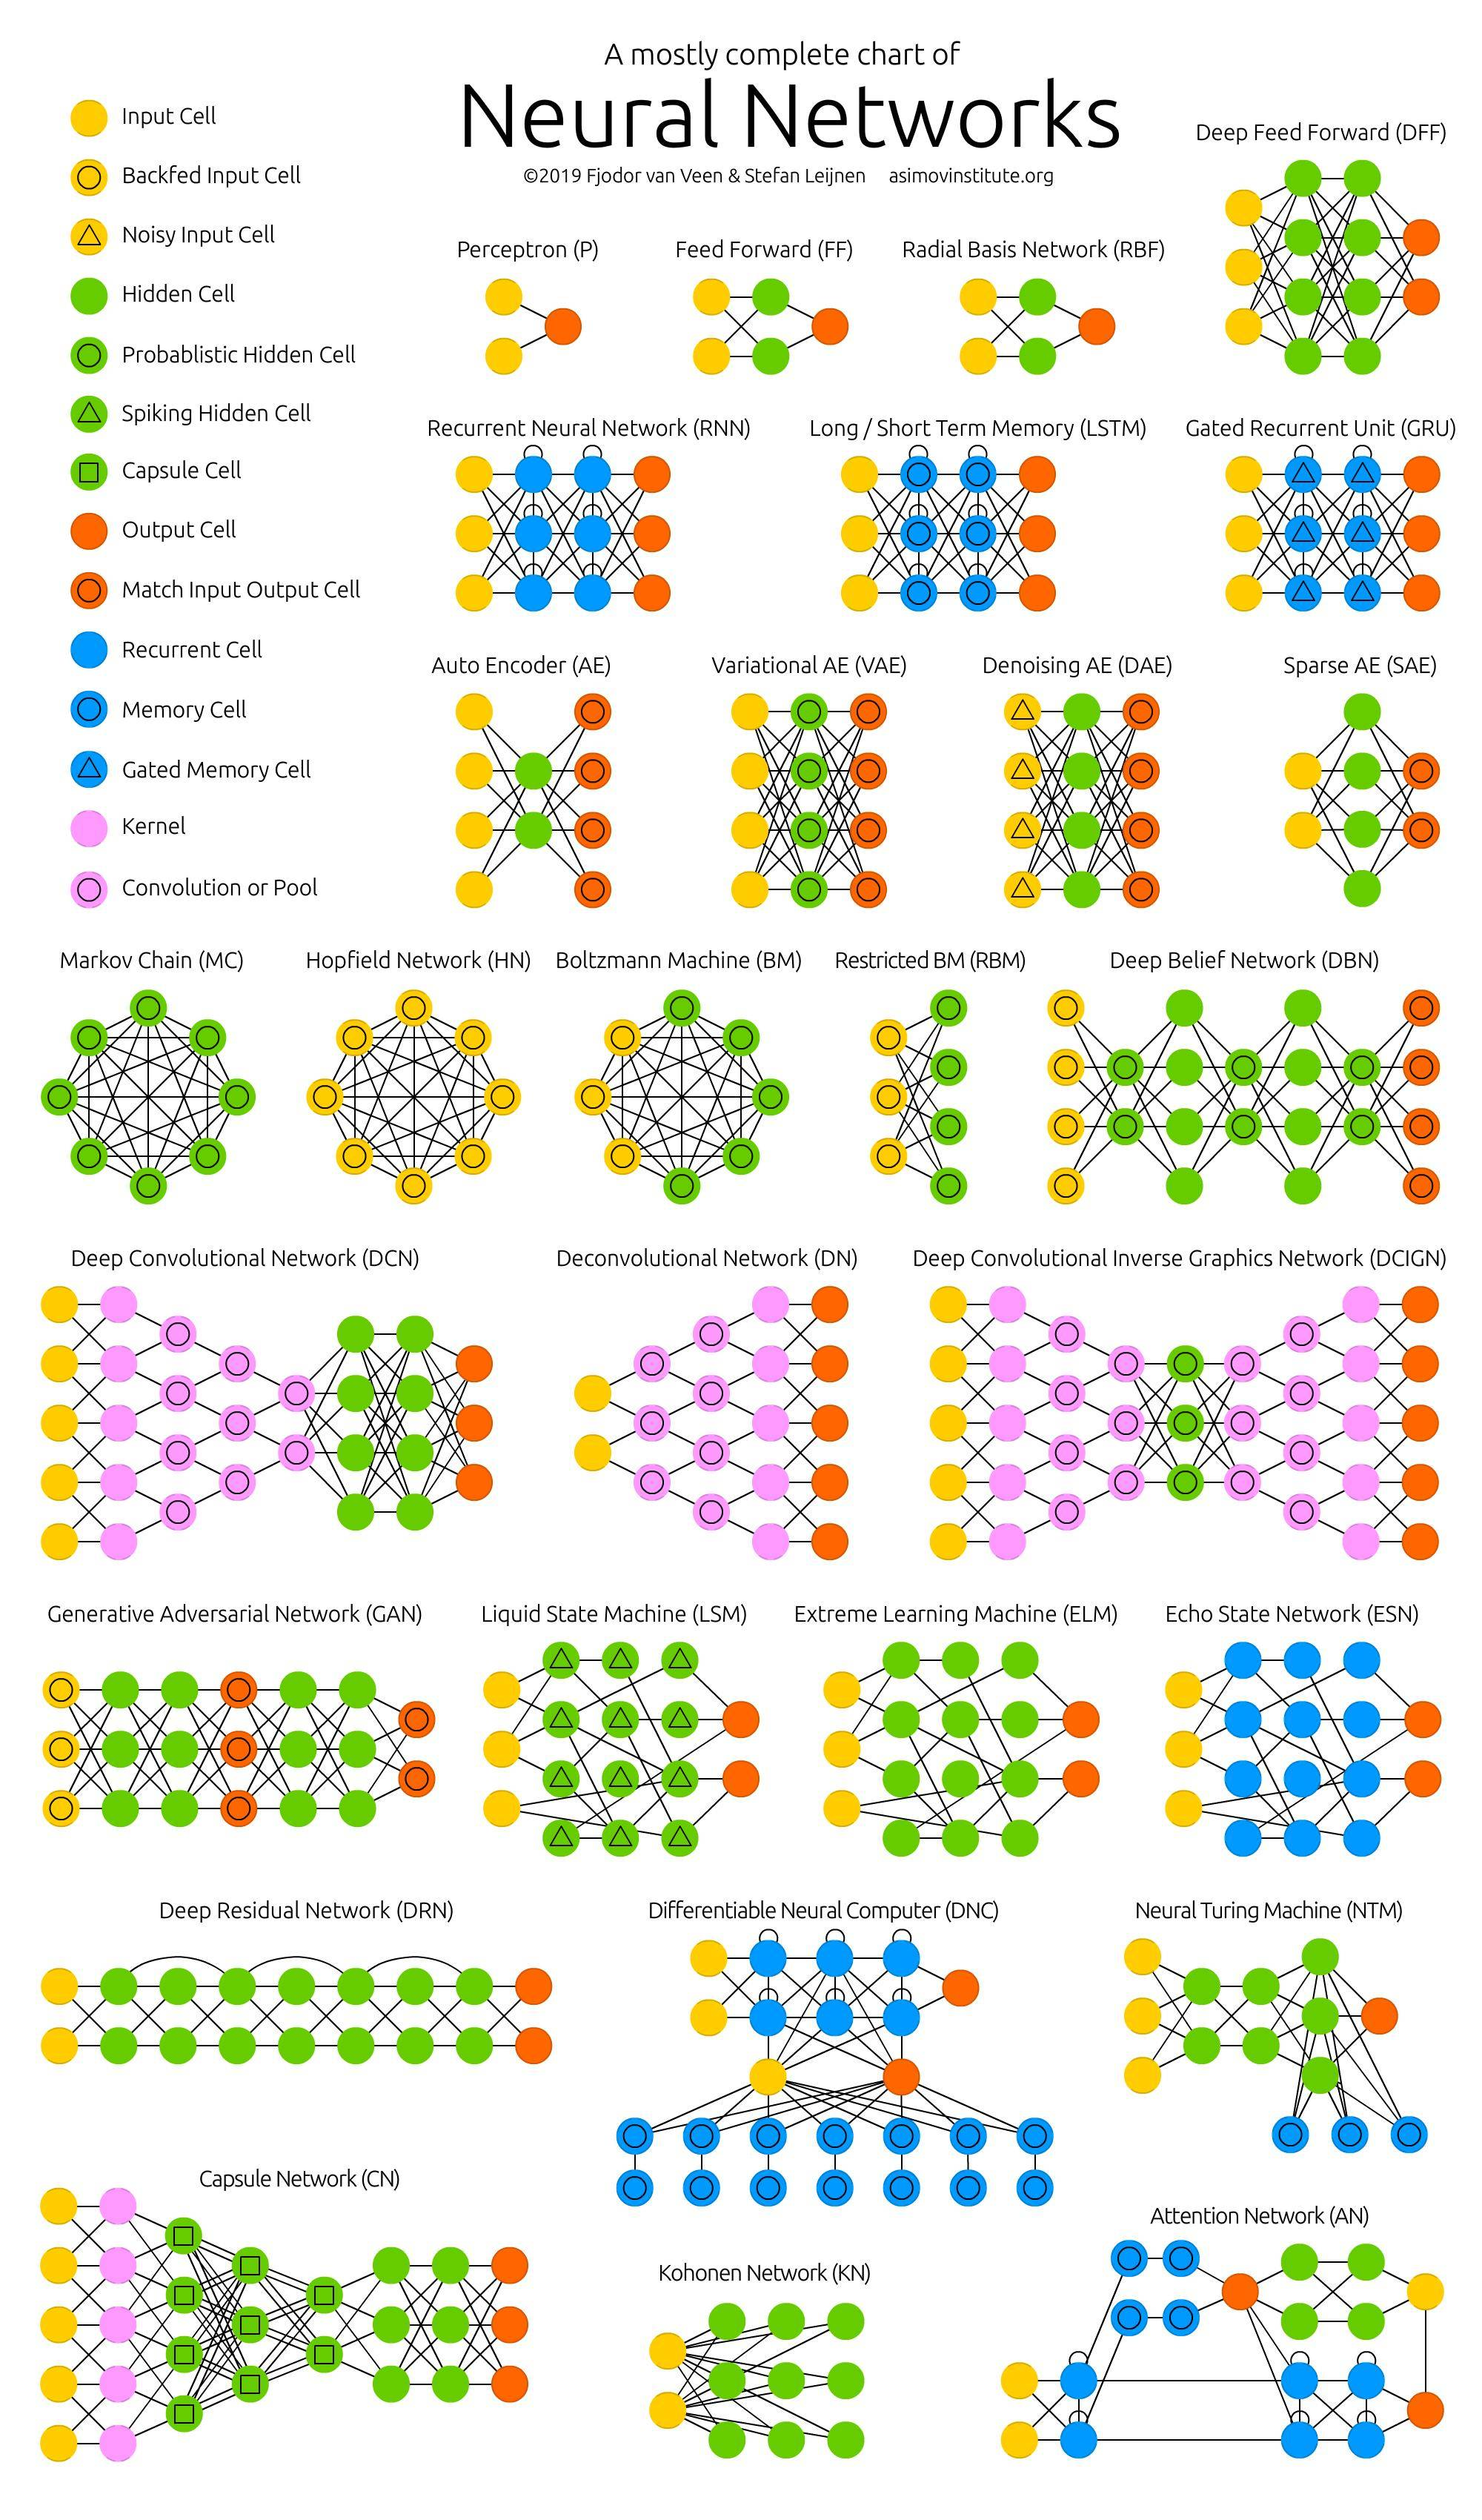
\includegraphics[scale = 0.1]{attachment/chapter_AML/Scc035}
	\caption{Types of artificial neural networks.}
\end{figure}

\paragraph{Concept Curve Fitting}
The \gls{AI_NN} fits its internal parameters to such a degree that the training data, given the parameters of the \gls{AI_NN}, produce an output that "fits" the required output.\\

For example, if the training data output or target values $\vec{y}$ represent a sinusoidal curve, but the \gls{AI_NN} produces linear output.
\begin{figure}[H]
	\centering
	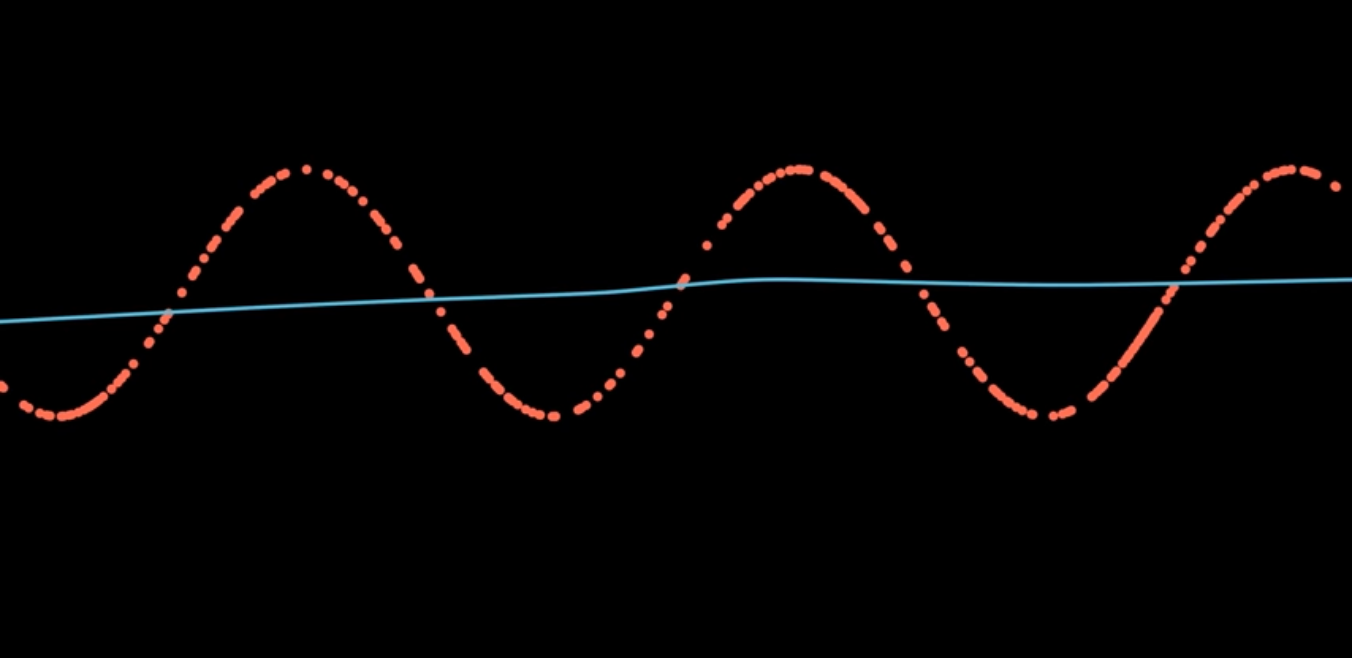
\includegraphics[scale = 0.2]{attachment/chapter_AML/Scc032}
	\caption{Curve fitting initial start}
\end{figure}

After some iterations of weight adjustments by the process of \textit{backpropagation} (a general term for \textit{gradient descent}), the \gls{AI_NN} reduces the loss value, and the output "fits" more closely to the target values.
\begin{figure}[H]
	\centering
	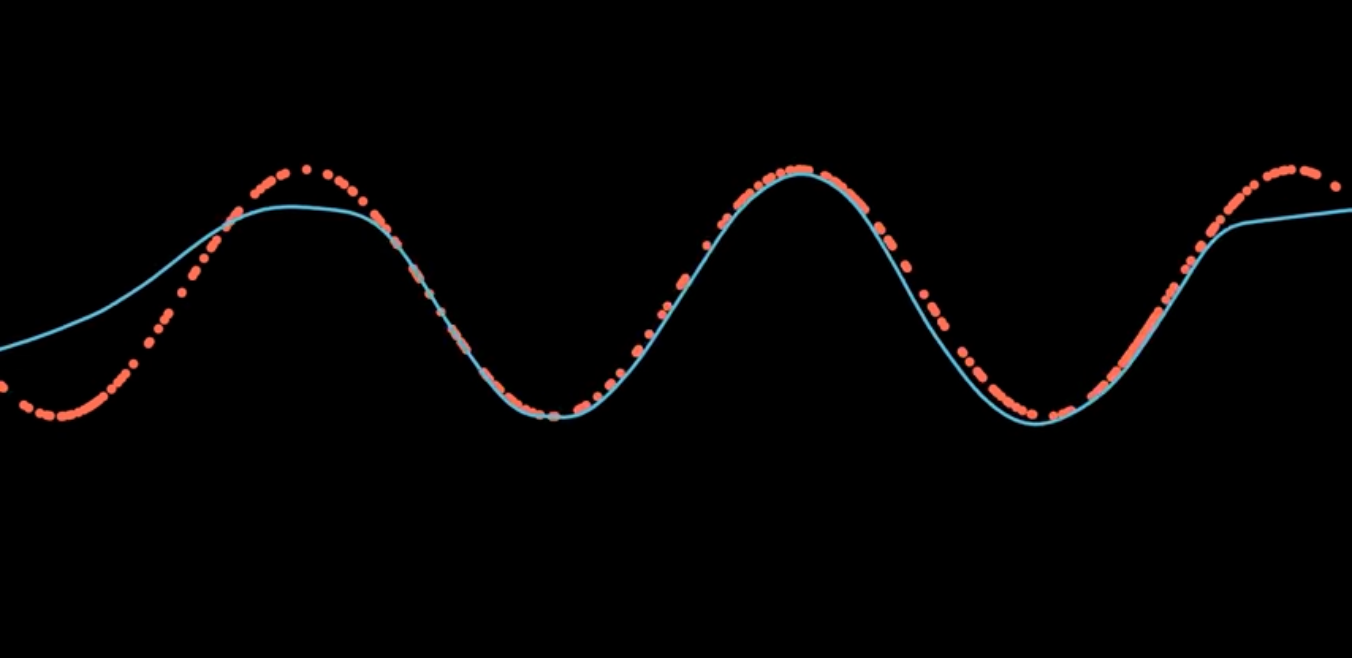
\includegraphics[scale = 0.2]{attachment/chapter_AML/Scc033}
	\caption{Curve fitting after some iterations}
\end{figure}

\begin{figure}[H]
	\centering
	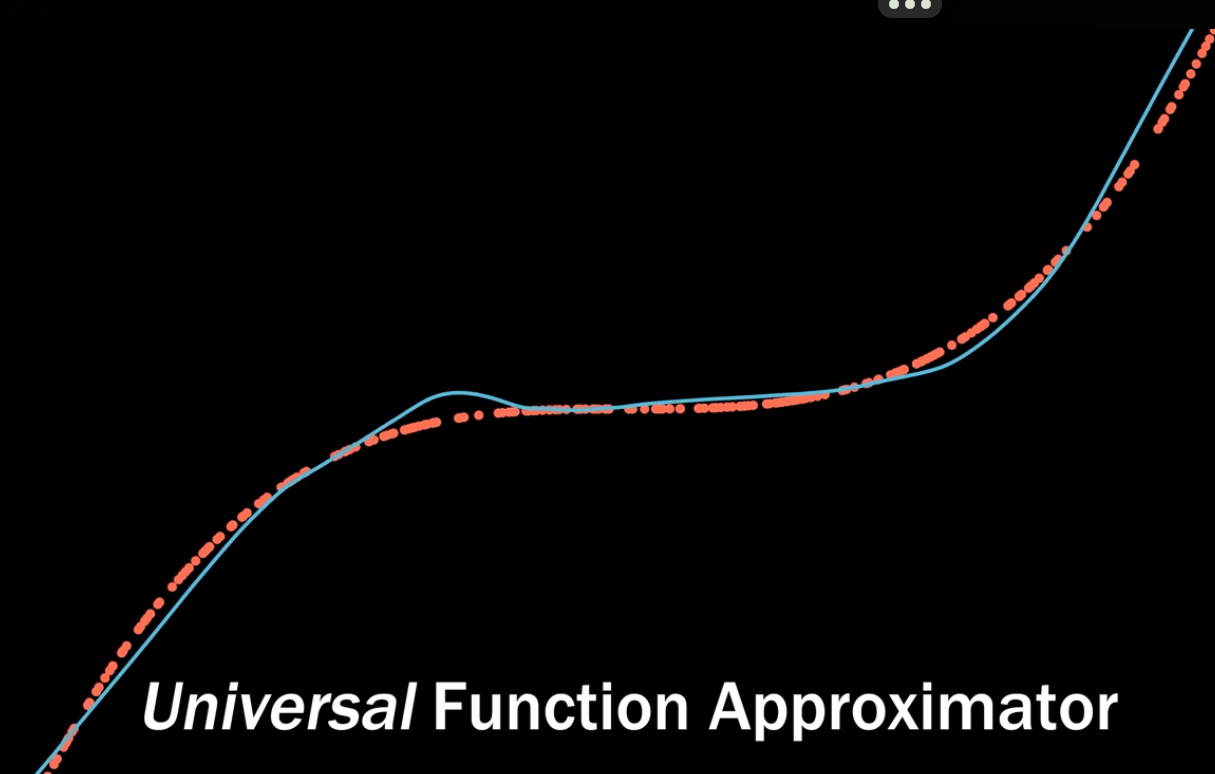
\includegraphics[scale = 0.2]{attachment/chapter_AML/Scc034}
	\caption{A Neural Net as a universal function approximator $f(x) \approx NN(x)$}
\end{figure}

\section{Theoretical Fundation}
\subsection{Multilayer Perceptrons (MLP)}

\paragraph{Mathematical Foundations}
Reference, siehe auskommentierte Link und dem Buch \cite{MLK_Andr_Buk}[93] % \href{https://www.mdpi.com/2075-1680/11/2/80#:~:text=Hence%2C%20each%20artificial%20neuron%20may,b%20)%20%2C%20see%20Figure%201.}{https://www.mdpi.com/2075-1680/11/2/80#:~:text=Hence%2C%20each%20artificial%20neuron%20may,b%20)%20%2C%20see%20Figure%201.}
\begin{description}
	\item \gls{AI_NN}: Nonlinear Mathematical Tools as Universal Function Approximators
	\item Each node combines an \textit{affine linear function} and a nonlinear \textit{activation function}. 
\end{description}

\glspl{AI_NN} are nonlinear mathematical tools\footnote{However, there is a possibility to design it so that it can be a linear function.}, intended to mimic human brain processes by stacking simple neurons together. The simplest unit of an \gls{AI_NN} is called a \textit{Neuron}. They are structured in \textit{layers}. The learning process for humans is called training, while for \glspl{AI_NN} it is referred to as training.

A layer can be represented as a \textit{parameterized function}. From the perspective of a directed graph, each node can be represented as an \textit{affine linear function}. The combination of each layer can be understood as a new \textit{affine linear function} [for a given neuron].

The nonlinear quality of an \gls{AI_NN} arises from the \textit{activation function}.

\paragraph{Transformer Function} Given the input $x^t$\footnote{
	The initial input of the layer can be understood as \textit{features}, which can be represented as a vector  $x^t = (x_1, \dots, x_n)$
}. These are processed in a \textit{neuron} through \textit{weights} $w_i, i=1,\dots, n$, producing $z$, which then produces the final output $y$ through some function $\phi$, $\phi(z) = y$.

The output $z$ is the result of processing the $n-x_i$ weightily:
\begin{align}
z &= (w_1, \dots, w_n) \left(\begin{matrix}
		x_1 \\
		\vdots \\
		x_n
	\end{matrix} \right) + b \\
  &= \sum_{i=1}^n x_i\cdot w_i +b = w^t x + b,
\end{align}
where $b$ is called \textit{bias}. This should give the system more flexibility by imitating a human filter. This \textit{affine function} can be changed into a linear function, where $b$ is set as $w_0$ and $x_0 = 1$:
\begin{align}
z &= (w_0, \dots, w_n) \left(\begin{matrix}
		x_0 = 1 \\
		\vdots \\
		x_n
	\end{matrix} \right) \\
  &= \sum_{i=0}^n x_i\cdot w_i = w^t x.
\end{align}
To avoid the notation of the transpose, it can be represented by $w\cdot x$.

However, depending on the needs, these processes can be viewed as affine or linear functions. In either case, processing the input $x_i$ resulting in $z$ is called a \textbf{transfer function}. Depending on the needs different transformers can be used. The most popular or most used is the sum operator $\sum$:

\begin{figure}[h]
\centering
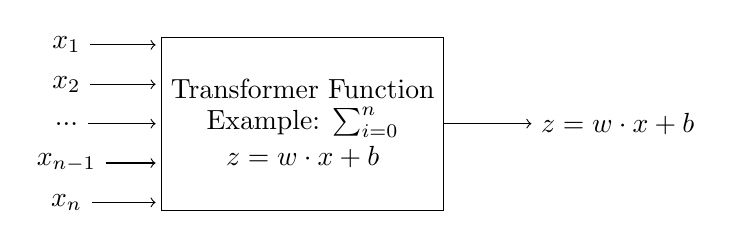
\begin{tikzpicture}
    % Nodes
    \foreach \x/\name in {1/x_1, 2/x_2, 3/. .. , 4/x_{n-1}, 5/x_n}
        \node at (0,-\x*0.5) (x\x) {$\name$};
  
    
    %% Node (e.g. Boxes, Symboles)    
    % Transformer Box
     \node[draw, minimum width=2cm, minimum height= 2.2 cm] at (3,-1.5) (transformer) {\shortstack{Transformer Function\\ Example: $\sum_{i=0}^n $\\ $z = w\cdot x + b$}};
    
    
    % Output activation symbole
    \node[right of=transformer, node distance=4cm] (z) {$z = w\cdot x + b$};
    
    
    %% Arrows
    % *0.5 reduces the distance
    \foreach \x in {1,2,...,5}*0.5
        \draw[->] (x\x.east) -- ([xshift=-2pt]transformer.west |- x\x);
    \draw[->] (transformer.east) -- (z.west);

    
\end{tikzpicture}
\caption{One perceptron, aka neuron}
\end{figure}

\paragraph{Activation Function}
The function $y=\phi(z)$ is known as the \textit{activation function} and it is this function that is resonsible for the non-linearity of the process. The function can be $"$freely$"$ selected, if it is fullyfilling certain criteria. \\

Each neuron can be regared as a mathematical function that is changing the \textit{transformation function} and the \textit{activation} with the inputs togehter: $y=\phi(z)= \phi\left(wx+b\right)$:

\begin{figure}[h]
\centering
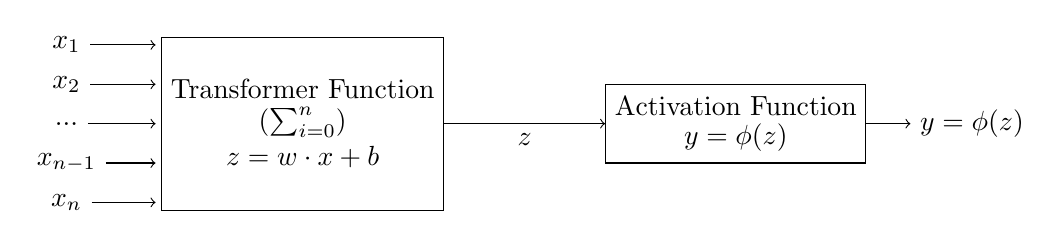
\begin{tikzpicture}
    % Nodes
    \foreach \x/\name in {1/x_1, 2/x_2, 3/. .. , 4/x_{n-1}, 5/x_n}
        \node at (0,-\x*0.5) (x\x) {$\name$};
  
    
    %% Node (e.g. Boxes, Symboles)
	 % Activation Box
    \node[draw, minimum width=2cm, minimum height= 1 cm] at (8.5,-1.5) (activation) {\shortstack{Activation Function \\ $y = \phi(z)$}};
    
    % Transformer Box
     \node[draw, minimum width=2cm, minimum height= 2.2 cm] at (3,-1.5) (transformer) {\shortstack{Transformer Function\\  $\left(\sum_{i=0}^n \right)$\\ $z = w\cdot x + b$}};
    
    
    % Output activation symbole
    \node[right of=activation, node distance=3cm] (phi) {$y = \phi(z) $};
    
    
    %% Arrows
    % *0.5 reduces the distance
    \foreach \x in {1,2,...,5}*0.5
        \draw[->] (x\x.east) -- ([xshift=-2pt]transformer.west |- x\x);
    \draw[->] (transformer.east) -- node[below] {$z$}(activation.west);
    \draw[->] (activation.east) -- (phi.west);

    
\end{tikzpicture}
\caption{One perceptron, aka neuron}
\end{figure}

\pagebreak
\paragraph{Feed-Forward}

As discussed before, the entirety of \glspl{AI_NN} can be understood as mathematical functions with an input $x$ and an output $y$.

\begin{align}
	f_{NN}(x) = y
\end{align} 

To combine each neuron, the output of each neuron is sent to all neurons in the next layer. This forwarding of information is called \textit{feed-forward}. From the perspective of a function, this is called \textit{verschachteln}. Each neuron in each layer (hidden layer) receives the output of the previous neurons. This neuron is then called a \gls{MLP}.

\begin{Definition}{Multilayer Perceptron}
	
	A \gls{MLP} is a function $f_l:\R^n \rightarrow \R$. It is called an $n-L-m$ perceptron, with $n$ inputs, $L$ hidden layers, and $m$ outputs.
	
	\begin{align}
		y = f^{(l)}(\vec{x}) = f_{l-1}\left(f_{l-2}\left(...\left(f_{0}(\vec{x})\right)\right)\right).
	\end{align}
	
	Where $f^{(i)}(\vec{z}) \stackrel{def}{=} \phi_l\left( \Matrix[W]^{(l)}\vec{z} + b^{(l)}\right)$.
\end{Definition}


\begin{figure}[h]
	\centering
\scalebox{0.6}{%
	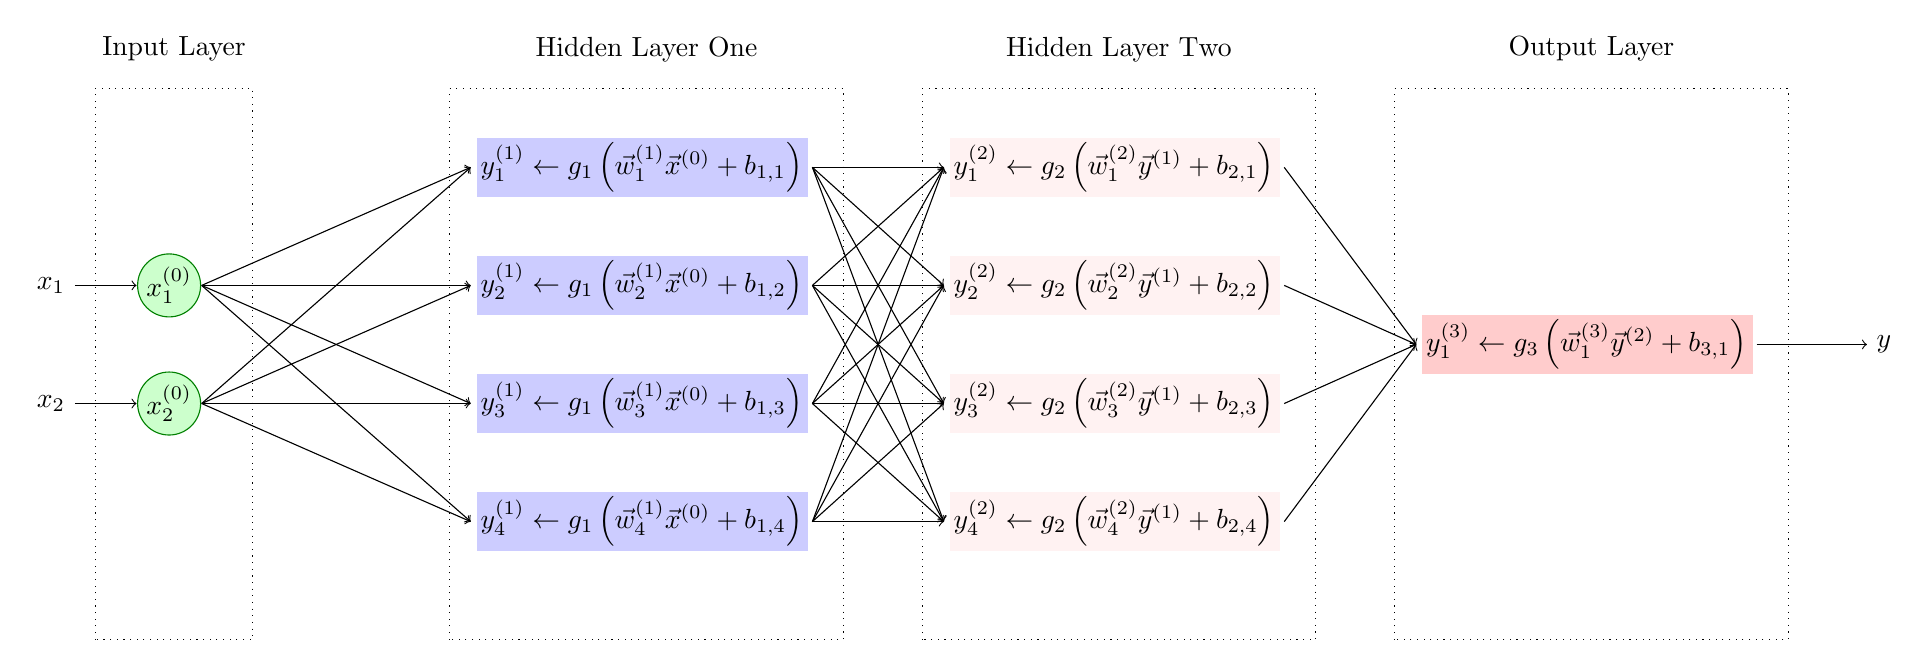
\begin{tikzpicture}
		
		% Drawing input on the left side each input layer
		\def\movefactorZeroZeroCircles{-7.5}
		\foreach \x/\layerindex in {1/x}{
			\foreach \y/\neuroindex in {6/1,4/2}{
				\node[name=\layerindex_\neuroindex] at (\x*3.25 +\movefactorZeroZeroCircles -0.8125,\y*0.75) {% function desciption
					$x_\neuroindex$
				};
				
			}
		}
		
		% Input layer with two neurons
		\draw[dotted] (-4.5,0) rectangle ++(2,7);
		\node at (-3.5,7.5) {Input Layer}; % Label for the Hidden layer one
		
		% Drawing circles on the left side of the Hidden layer one
		\def\movefactorZeroCircles{-6}
		\foreach \x/\layerindex in {1/0}{
			\foreach \y/\neuroindex in {6/1,4/2}{
				\filldraw[fill=green!20, draw=green!50!black] (\x*3.25 +\movefactorZeroCircles -0.8125,\y*0.75) circle circle (0.4);
				\node[name=\layerindex_\neuroindex] at (\x*3.25 +\movefactorZeroCircles -0.8125,\y*0.75) {% function desciption
					$x^{(\layerindex)}_{\neuroindex}$
				};
			}
		}   
		
		% Hidden layer one with four neurons
		\draw[dotted] (0,0) rectangle ++(5,7);
		\node at (2.5,7.5) {Hidden Layer One}; % Label for the Hidden layer one
		
		% Drawing neurons and displaying function in the Hidden layer one
		\foreach \x/\layerindex in {1/1}{
			\def\forwardedlayerindex{0}
			\foreach \y/\neuroindex in {8/1,6/2,4/3,2/4}{
				\fill[blue!20] (\x*3.25 -2.9,\y*0.75-0.375) rectangle ++(4.2,0.75);
				\node[name=\layerindex_\neuroindex] at (\x*3.25-0.8125,\y*0.75-0.375+0.375) {% function desciption
					$y_\neuroindex^{(\layerindex)} \leftarrow g_\layerindex \left(\vec{w}^{(\layerindex)}_{\neuroindex}\vec{x}^{(\forwardedlayerindex)}+b_{\layerindex,\neuroindex}\right)$
				};
			}
		}
		
		% Second box with four neurons
		\draw[dotted] (6,0) rectangle ++(5,7);
		\node at (8.5,7.5) {Hidden Layer Two}; % Label for the second box
		
		% Drawing neurons and displaying function in the second box
		\def\movefactorSecondBox{6}
		\def\forwardedlayerindex{1}
		\foreach \x/\layerindex in {1/2}{
			\foreach \y/\neuroindex in {8/1,6/2,4/3,2/4}{
				\fill[pink!20] (\x*3.25 + \movefactorSecondBox -2.9,\y*0.75-0.375) rectangle ++(4.2,0.75);
				\node[name=\layerindex_\neuroindex] at (\x*3.25+ \movefactorSecondBox -0.8125,\y*0.75-0.375+0.375) {% function desciption
					$y_\neuroindex^{(\layerindex)} \leftarrow g_\layerindex \left(\vec{w}^{(\layerindex)}_{\neuroindex}\vec{y}^{(\forwardedlayerindex)}+b_{\layerindex,\neuroindex}\right)$
				};
			}
		}
		
		% Third box with a single inner box
		\draw[dotted] (12,0) rectangle ++(5,7);
		\node at (14.5,7.5) {Output Layer}; % Label for the third box
		
		% Drawing neurons and displaying function in the third box
		\def\movefactorThirdBox{6}
		\def\forwardedlayerindex{2}
		\foreach \x/\layerindex in {1/3}{
			\foreach \y/\neuroindex in {5/1}{
				\fill[red!20] (\x*3.25 + \movefactorSecondBox + \movefactorThirdBox -2.9,\y*0.75-0.375) rectangle ++(4.2,0.75);
				\node[name=\layerindex_\neuroindex] at (\x*3.25+ \movefactorSecondBox + \movefactorThirdBox -0.8125,\y*0.75-0.375+0.375) {% function desciption
					$y_\neuroindex^{(\layerindex)} \leftarrow g_\layerindex \left(\vec{w}^{(\layerindex)}_{\neuroindex}\vec{y}^{(\forwardedlayerindex)}+b_{\layerindex,\neuroindex}\right)$
				};
			}
		}
		
		% Arrows connecting right side of input to left side of the corresponding cicle
		\draw[->] (x_1) -- (0_1);
		\draw[->] (x_2) -- (0_2);
		
		% Arrows connecting right side of circels to left side of the corresponding inner box of the Hidden layer one
		\foreach \x in {1,2}
		\foreach \y in {1,2,3,4}
		\draw[->] (0_\x.east) -- (1_\y.west);
		
		
		% Arrows connecting right side of neurons of the Hidden layer one to left side of the corresponding inner box of the second box
		\foreach \x in {1,2,3,4}
		\foreach \y in {1,2,3,4}
		\draw[->] (1_\x.east) -- (2_\y.west);
		
		% Arrows connecting right side of neurons of the second box to left side of the single inner box of the third box
		\foreach \x in {1,2,3,4}
		\foreach \y in {1}
		\draw[->] (2_\x.east) -- (3_\y.west);
		
		% Arrow from right side of inner box of the third box to slightly outside the dotted line with label y on the right hand side
		\draw[->] (3_1.east) -- (6+\movefactorSecondBox+\movefactorThirdBox,5*0.75) node[right] {$y$};
		
		
		
	\end{tikzpicture}
}
\caption{\gls{MLP} with two hidden layer, one input vector and one output layer}
\end{figure}


In this example, the output of the \gls{MLP} $y^{(1)}_1$ is calculated by the activation function $g_1$ for the hidden layer $1$. The weight vector $\vec{w}^{(0)}_1$ has dimension $2$, as it receives two inputs $x^{(1)}_1$ and $x^{(1)}_2$, along with the scalar bias $b^{(1)}_1$. In the next layer, the dimension of each weight vector is $4$, as each \gls{MLP} receives inputs $y^{(1)}_1$, $y^{(1)}_2$, $y^{(1)}_3$, and $y^{(1)}_4$ from the previous layer.

\subsection{Activation Function}
\paragraph*{Sigmoid Function}
The sigmoid activation function is on of the well know activation function. It's characteristic $S-$Shape is bound between the $1$ and $0$:

\begin{align}
	\sigma(x) = \frac{1}{1+e{-x}}	
\end{align}


\begin{lstlisting}[language=iPython, caption={Example code to create a Sigmoid Function}]
# Sigmoid function in Python
import matplotlib.pyplot as plt
import numpy as np

x = np.linspace(-5, 5, 50)
z = 1/(1 + np.exp(-x))

plt.subplots(figsize=(8, 5))
plt.plot(x, z)
plt.grid()
plt.show()
\end{lstlisting}


\begin{figure}[h]
	\centering
\scalebox{0.6}{%
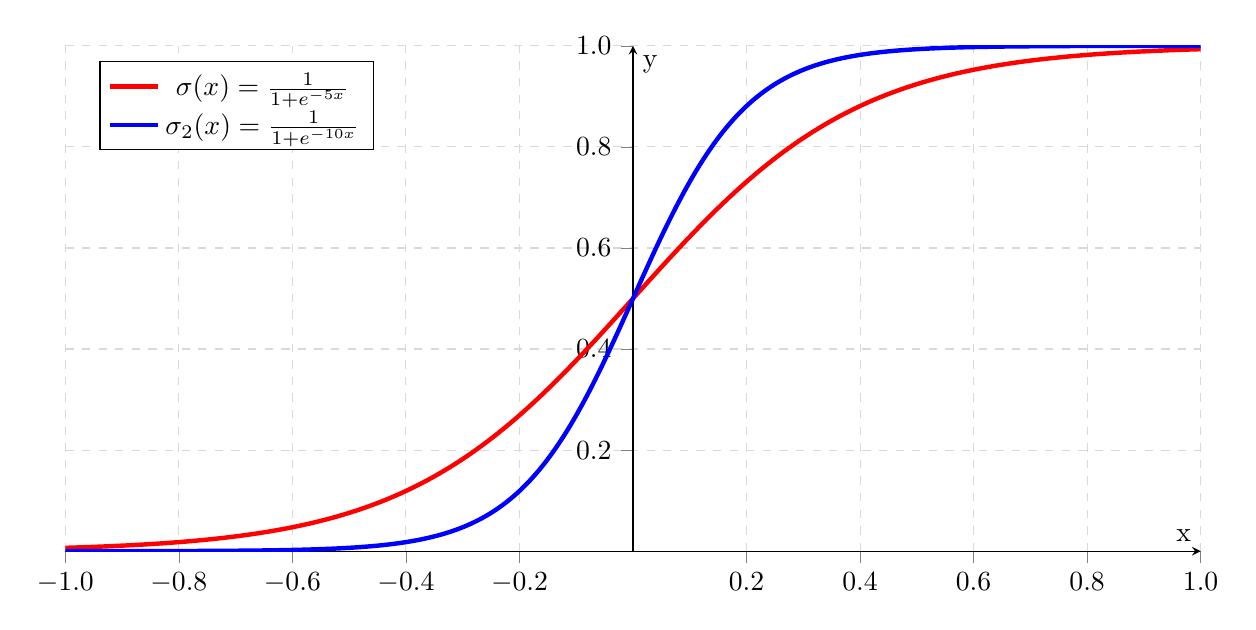
\begin{tikzpicture}
    \begin{axis}[
    	legend pos=north west,
        axis x line=middle,
        axis y line=middle,
        x tick label style={/pgf/number format/fixed,
                            /pgf/number format/fixed zerofill,
                            /pgf/number format/precision=1},
        y tick label style={/pgf/number format/fixed,
                            /pgf/number format/fixed zerofill,
                            /pgf/number format/precision=1},
        grid = major,
        width=16cm,
        height=8cm,
        grid style={dashed, gray!30},
        xmin=-1,     % start the diagram at this x-coordinate
        xmax= 1,    % end   the diagram at this x-coordinate
        ymin= 0,     % start the diagram at this y-coordinate
        ymax= 1,   % end   the diagram at this y-coordinate
        %axis background/.style={fill=white},
        xlabel=x,
        ylabel=y,
        tick align=outside,
        enlargelimits=false]
      % plot the stirling-formulae
      \addplot[domain=-1:1, red, ultra thick,samples=500] {1/(1+exp(-5*x))};
      \addplot[domain=-1:1, blue, ultra thick,samples=500] {1/(1+exp(-10*x))};
      \addlegendentry{$\sigma(x)=\frac{1}{1+e^{-5x}}$}
      \addlegendentry{$\sigma_2(x)=\frac{1}{1+e^{-10x}}$}
    \end{axis}
\end{tikzpicture}
}
\caption{Example of two sigmoid functions}
\end{figure}

\paragraph*{Tanh}
This is also a hyperbolic S-shape curves like the sigmoid function. It's bound between $-1$ and $1$.

\begin{align}
	\tanh(x) = \frac{1-e^{-x}}{1+e{-x}}
\end{align}


\begin{figure}[h]
	\centering
\scalebox{0.6}{%
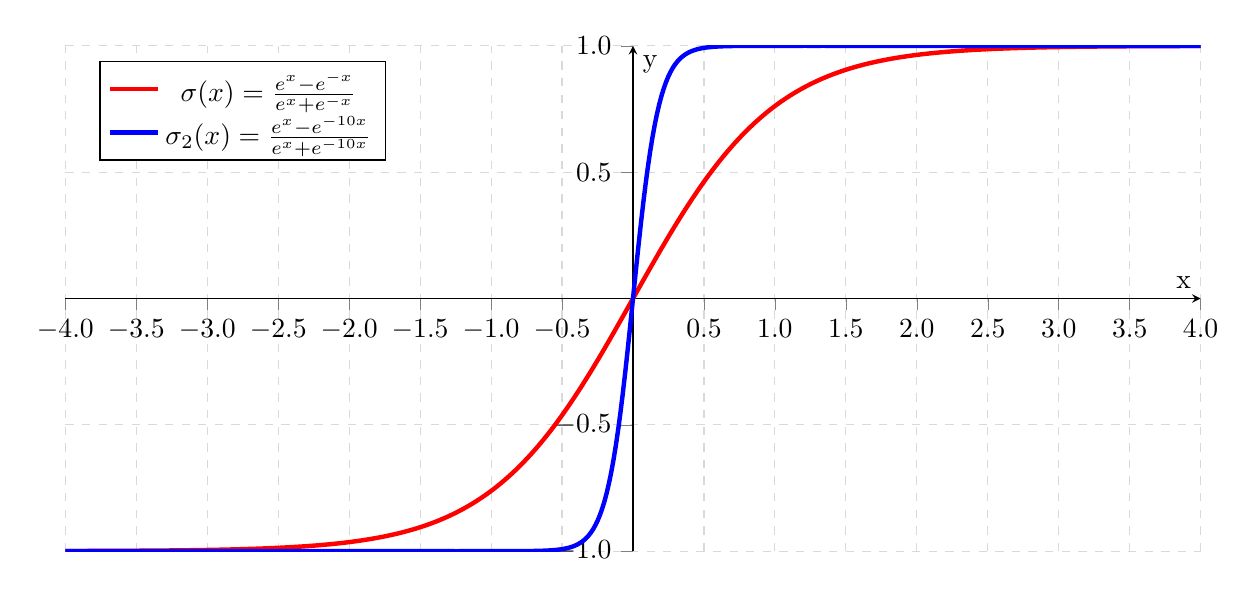
\begin{tikzpicture}
    \begin{axis}[
    	legend pos=north west,
        axis x line=middle,
        axis y line=middle,
        x tick label style={/pgf/number format/fixed,
                            /pgf/number format/fixed zerofill,
                            /pgf/number format/precision=1},
        y tick label style={/pgf/number format/fixed,
                            /pgf/number format/fixed zerofill,
                            /pgf/number format/precision=1},
        grid = major,
        width=16cm,
        height=8cm,
        grid style={dashed, gray!30},
        xmin=-4,     % start the diagram at this x-coordinate
        xmax= 4,    % end   the diagram at this x-coordinate
        ymin= -1,     % start the diagram at this y-coordinate
        ymax= 1,   % end   the diagram at this y-coordinate
        %axis background/.style={fill=white},
        xlabel=x,
        ylabel=y,
        tick align=outside,
        enlargelimits=false]
      % plot the stirling-formulae
      \addplot[domain=-4:4, red, ultra thick,samples=500] {(exp(x) -exp(-x)) /(exp(x)+exp(-x))};
      \addplot[domain=-4:4, blue, ultra thick,samples=500] {(exp(x) -exp(-10*x)) /(exp(x)+exp(-10*x))};
      \addlegendentry{$\sigma(x)=\frac{e^x-e^{-x}}{e^x+e^{-x}}$}
      \addlegendentry{$\sigma_2(x)=\frac{e^x-e^{-10x}}{e^x+e^{-10x}}$}
    \end{axis}
\end{tikzpicture}
}
\caption{Example of two tanh}
% Source: https://github.com/MartinThoma/LaTeX-examples/blob/master/tikz/sigmoid-function/sigmoid-function.tex
\end{figure}

\paragraph{Softmax}
The softmax activation function most commenly used for the outputlayer. In ingest multiple inputs onto the intervall of $0$ and $1$. The output of the softmax function can then be used to represent a probability distribution.
\begin{align}
	softmax(x) = \frac{e^x}{\sum e^{x_i}}
\end{align}

\paragraph{ReLu}
The \gls{ReLU} action function is offen the default activation function for several neural networks.\\

Using the sigmoid or tanh function to build deep neural networks is risky since they are more likely to suffer from the vanishing gradient problem.\footnote{
	The \textit{vanishing gradient problem} is the problem, where the gradient for the weights in early layers of the network is very small. This inturn will reduce the change of the weights to find a better small loss value.
}
\begin{align}
	ReLu(x) = x^+ = \max(0,x) = \frac{x + \mid x \mid}{2} = \begin{cases}
	x,& \text{if } x> 0\\
    0,& \text{otherwise}
\end{cases}
\end{align}

\begin{lstlisting}[language=iPython, caption={Example code to create a ReLU}]

# ReLU in Python
import matplotlib.pyplot as plt
import numpy as np

x = np.linspace(-5, 5, 50)
z = [max(0, i) for i in x]

plt.subplots(figsize=(8, 5))
plt.plot(x, z)
plt.grid()
plt.show()

\end{lstlisting}

\begin{figure}[h]
	\centering
\scalebox{0.6}{%

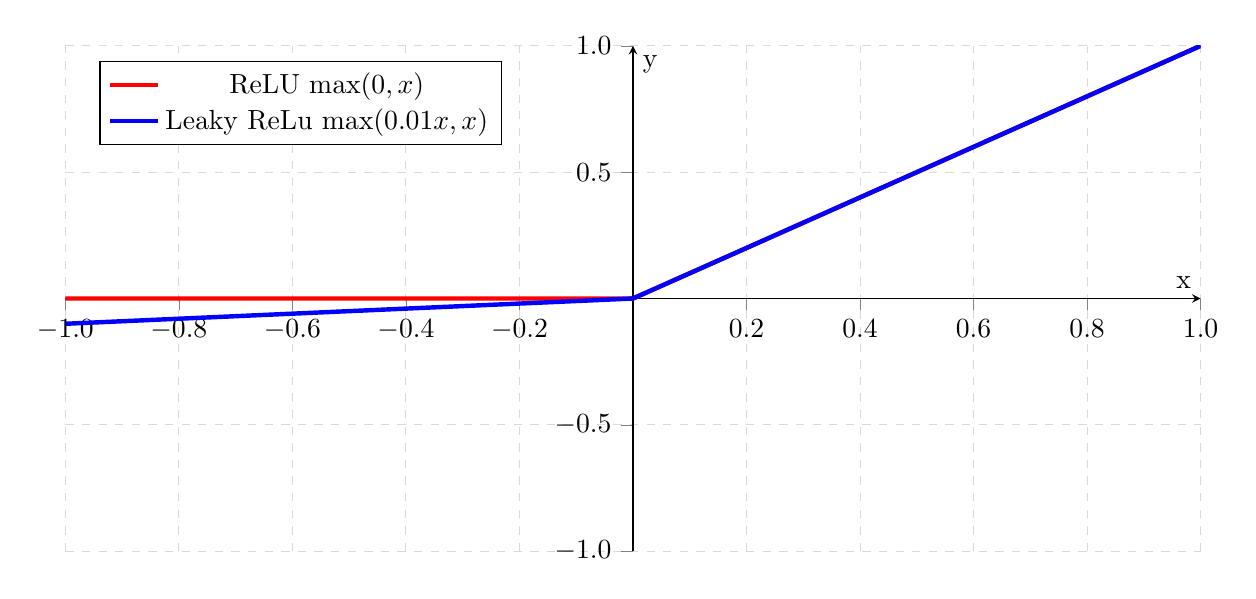
\begin{tikzpicture}
    \begin{axis}[
    	legend pos=north west,
        axis x line=middle,
        axis y line=middle,
        x tick label style={/pgf/number format/fixed,
                            /pgf/number format/fixed zerofill,
                            /pgf/number format/precision=1},
        y tick label style={/pgf/number format/fixed,
                            /pgf/number format/fixed zerofill,
                            /pgf/number format/precision=1},
        grid = major,
        width=16cm,
        height=8cm,
        grid style={dashed, gray!30},
        xmin=-1,     % start the diagram at this x-coordinate
        xmax= 1,    % end   the diagram at this x-coordinate
        ymin= -1,     % start the diagram at this y-coordinate
        ymax= 1,   % end   the diagram at this y-coordinate
        %axis background/.style={fill=white},
        xlabel=x,
        ylabel=y,
        tick align=outside,
        enlargelimits=false]
      % plot the stirling-formulae
      \addplot[domain=-1:1, red, ultra thick,samples=500] {max(0,x)};
      \addplot[domain=-1:1, blue, ultra thick,samples=500] {max(0.1*x,x)};
      \addlegendentry{ReLU $\max(0,x)$};
      \addlegendentry{Leaky ReLu $\max(0.01x,x)$};
 \end{axis}
\end{tikzpicture}
}
\caption{Example of two tanh}
% Source: https://github.com/MartinThoma/LaTeX-examples/blob/master/tikz/sigmoid-function/sigmoid-function.tex
\end{figure}
	
\subsection{Optimization (Calculus)}
\paragraph{Stochastic Gradient Descent}
We now consider the problem of solving for the \textit{minimum} of a real-values function
\begin{align}
	\min_{x} 	f_{NN}(x).
\end{align}
For example, we assume
\begin{itemize}
	\item $	f_{NN}:\R-^4 \rightarrow R$ captures the machine learning problem at hand,
	\item $f_{NN}$ is differentiable,
	\item we are unable to analytically find the solution in closed form.
\end{itemize}
The \textit{gradient descent} takes steps a proportionaly ($\gamma$) to the negative of the gradient of the function $\nabla 	f_{NN}$ at the current point $x_0$:
\begin{align}
	\nabla x_1 = x_0 - \gamma ((\nabla 	f_{NN})(x_0))^T.
\end{align}
At the point $x_0$ the function $	f_{NN}(x_0)$ degresses fastes if on moves from $x_0$ in the direction of the negative gradient $- \gamma ((\nabla 	f_{NN})(x_0))^T$ of $f_{NN}$ at $x_0$. From this follows: For a small \textit{step-size}\footnote{In Azure ML is called \textit{learning-rate}} $\gamma \geq 0$ $	f_{NN}(x_1)\geq 	f_{NN}(x_0)$.\\


To find the \underline{local} optimum $f_{x_*}$ we start with a inial guess $x_0$ of the parameter we wish to optimize. Then we iterate according to 

\begin{align}
	\nabla x_{i+1} = x_i - \gamma_i ((\nabla f)(x_i))^T.
\end{align}
For a suitable step-size $\gamma_i$, the sequence $f(x_0)\leq f(x_1) \leq ... $ converges to a \textit{local} minimum.

Only if the step-size $\gamma$ is a big, that the $f(x_{i+1}$ overshots the local minimum, the functional value $y=f(x_{i})$ converges to the local minimum.

\begin{figure}[H]
	\centering
	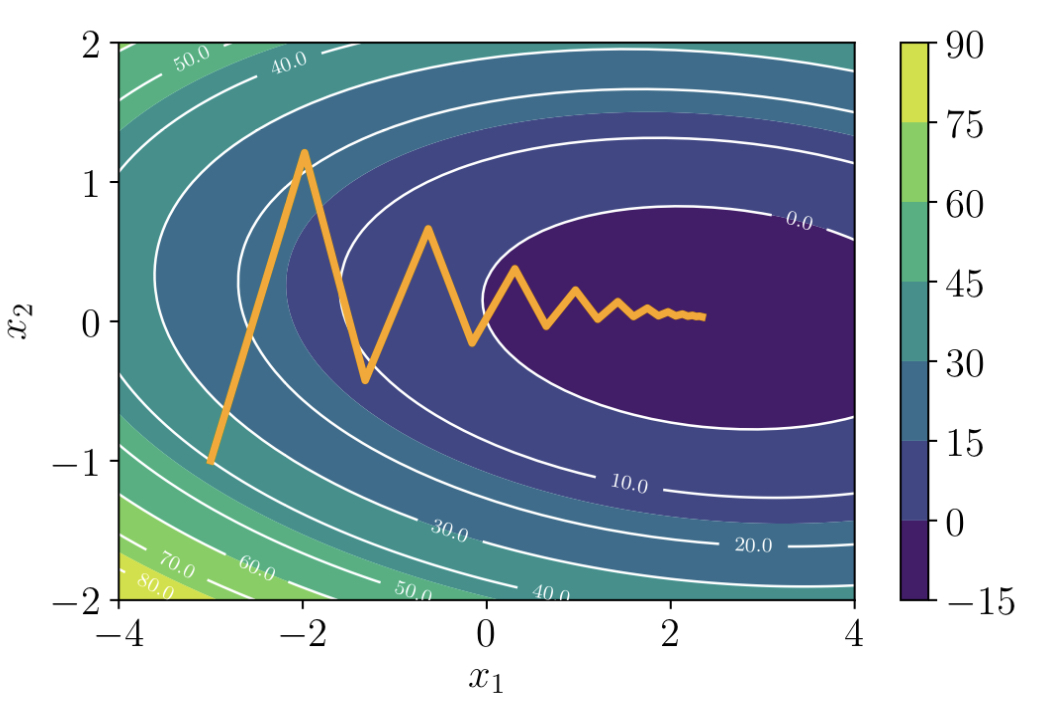
\includegraphics[scale = 0.2]{attachment/chapter_10/Scc053}
	\caption{Graph shows the gradient descent on a two dimensional quadratic surface.}
\end{figure}

\paragraph{Epoch}
%Unclear, what is an iteration.

Let's assume we have 1000 datasets, where each dataset has collection of features and a target value. An \gls{g_Epoch}

%\begin{figure}[H]
%	\centering
%	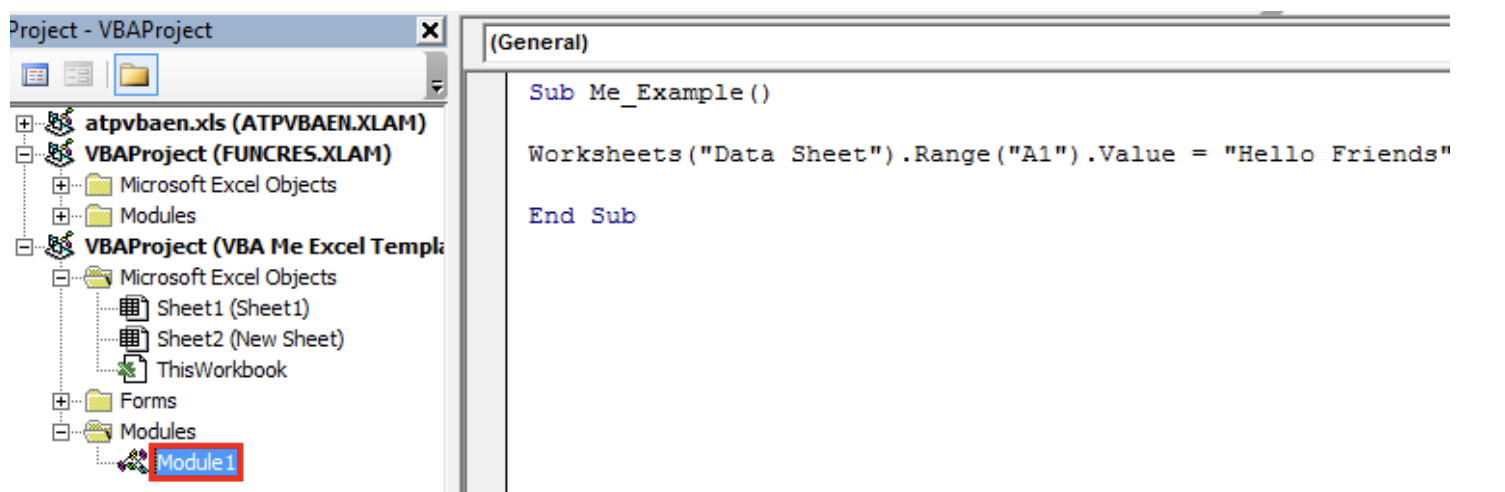
\includegraphics[scale = 0.2]{attachment/chapter_10/Scc054}
%	\caption{gjhg}
%\end{figure}

\section{Building a Simple Architecture}
\subsection{Tensor}

What it means to represent and organize data in a \textit{tensor} can be viewed for \gls{ML} as two different concepts.
\begin{description}
    \item[Data Storage] Multidimensional Arrays/data tensor. Note: Arrays are not matrices. For example, a scalar is zero-dimensional, a vector is one-dimensional, a matrix is two-dimensional, and so on. This concept is used to store data, depending on the relationship.
    \item[Multilinear Mapping (Mathematical object)] This may express a multilinear relationship between a set of algebraic objects.
\end{description}
The data tensor may be analyzed or preprocessed either by tensor methods, which rely on tensor methods like decomposition that are rooted in the understanding of tensors as multilinear mapping. Through \gls{AI_NN}, these data tensors or preprocessed data tensors can be further analyzed.\\
% See https://tspace.library.utoronto.ca/bitstream/1807/65327/11/Vasilescu_M_Alex_O_200911_PhD_thesis.pdf#page44
% See https://en.wikipedia.org/wiki/Tensor_(machine_learning)

In \textit{PyTorch} a \textit{tensor} is data abstraction, aka data tensor. The relevant module for this is $\verb|torch|$. By using $\verb|torch.empty(3,4)|$ a tensor has 3 expression for the first dimension and 4 for the second dimension. Note: $\verb|torch.empty(1)| $ creates a tensor equal to a scalar object. $\verb|torch.empty(3)|$  a vector and $\verb|torch.empty(2,2)|$ a matrix, and $\verb|torch.empty(3,3,3)|$ a higher dimensional object.


\subsection{nn.Linear}
\paragraph{Releated Field}
This module is fundamental in PyTorch, not only for \gls{AI_NN}. $\verb|nn.Linear|$ is a linear layer, that applies a lineare transformation to input data using \textit{weights} and \textit{biases}.\\

This module find versatial application
\begin{itemize}
	\item[\gls{FFNN}] This kind of networks are fully connected with at lest three layers. The module $\verb|nn.linear|$ is used to implement this connection.
	\item[Linear Regression] In this case the module can be used to model the linear implementation of the equation.
	\item[Data Transformation] In case the data need to be transformed into higher dimenension, then his module can help
	\item[Further deep learning architecture] For example modules like Autoencoder using this module as well. 
\end{itemize}

Related or further topics:
\begin{itemize}
	\item Comparing nn.Linear and nn.Conv2d. Whiche nn.Linear applies a linear transformation the nn.Conv2d a 2D convoluation. % https://docs.kanaries.net/topics/Python/nn-linear
\end{itemize}

\paragraph{Weight Matrix}
Each node $n^{(j)}_i$ in layer $j$ has an output $y^{(j)}_i$, where 
\begin{itemize}
    \item[$j$] Index for the layer,
    \item[$i$] Index for the node in layer $j$,
    \item[$y$] Output of node $i$ in layer $j$.
\end{itemize}

In the example, layer 1 has four nodes, therefore the outputs are
\begin{align}
    y^{(1)}_1, \dots, y^{(1)}_4.
\end{align}

\begin{figure}[h]
	\centering
\scalebox{0.6}{%

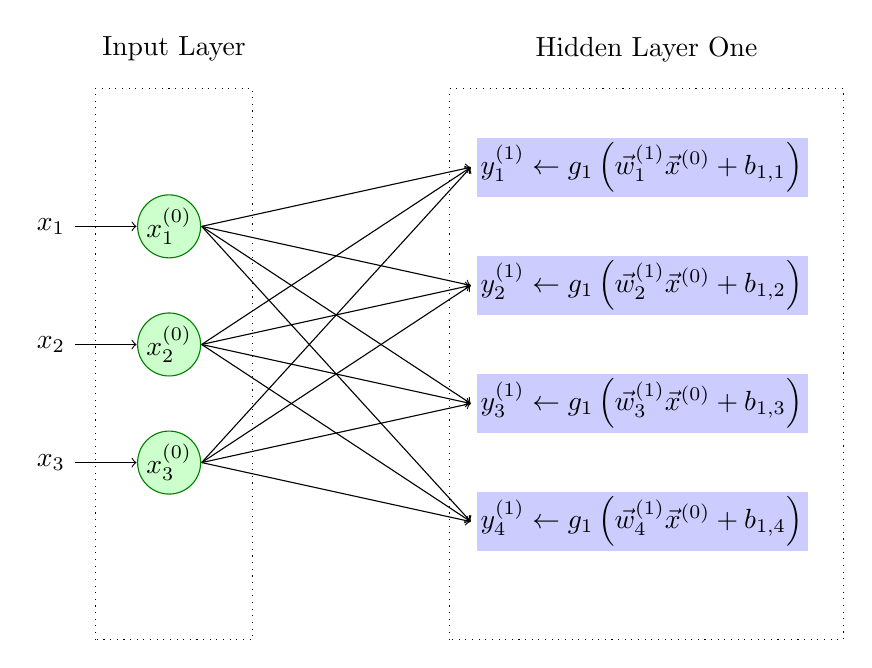
\begin{tikzpicture}
		
		% Drawing input on the left side each input layer
		\def\movefactorZeroZeroCircles{-7.5}
		\foreach \x/\layerindex in {1/x}{
			\foreach \y/\neuroindex in {7/1,5/2, 3/3}{
				\node[name=\layerindex_\neuroindex] at (\x*3.25 +\movefactorZeroZeroCircles -0.8125,\y*0.75) {% function desciption
					$x_\neuroindex$
				};
				
			}
		}
		
		% Input layer with two neurons
		\draw[dotted] (-4.5,0) rectangle ++(2,7);
		\node at (-3.5,7.5) {Input Layer}; % Label for the Hidden layer one
		
		% Drawing circles on the left side of the Hidden layer one
		\def\movefactorZeroCircles{-6}
		\foreach \x/\layerindex in {1/0}{
			\foreach \y/\neuroindex in {7/1,5/2, 3/3}{
				\filldraw[fill=green!20, draw=green!50!black] (\x*3.25 +\movefactorZeroCircles -0.8125,\y*0.75) circle circle (0.4);
				\node[name=\layerindex_\neuroindex] at (\x*3.25 +\movefactorZeroCircles -0.8125,\y*0.75) {% function desciption
					$x^{(\layerindex)}_{\neuroindex}$
				};
			}
		}   
		
		% Hidden layer one with four neurons
		\draw[dotted] (0,0) rectangle ++(5,7);
		\node at (2.5,7.5) {Hidden Layer One}; % Label for the Hidden layer one
		
		% Drawing neurons and displaying function in the Hidden layer one
		\foreach \x/\layerindex in {1/1}{
			\def\forwardedlayerindex{0}
			\foreach \y/\neuroindex in {8/1,6/2,4/3,2/4}{
				\fill[blue!20] (\x*3.25 -2.9,\y*0.75-0.375) rectangle ++(4.2,0.75);
				\node[name=\layerindex_\neuroindex] at (\x*3.25-0.8125,\y*0.75-0.375+0.375) {% function desciption
					$y_\neuroindex^{(\layerindex)} \leftarrow g_\layerindex \left(\vec{w}^{(\layerindex)}_{\neuroindex}\vec{x}^{(\forwardedlayerindex)}+b_{\layerindex,\neuroindex}\right)$
				};
			}
		}
		
		
		
		% Arrows connecting right side of input to left side of the corresponding cicle
		\draw[->] (x_1) -- (0_1);
		\draw[->] (x_2) -- (0_2);
		\draw[->] (x_3) -- (0_3);
		
		
		% Arrows connecting right side of circels to left side of the corresponding inner box of the Hidden layer one
		\foreach \x in {1,2,3}
		\foreach \y in {1,2,3,4}
		\draw[->] (0_\x.east) -- (1_\y.west);
				
		
	\end{tikzpicture}

}
\caption{Example Two Layer Network}
\end{figure}

In a \gls{FFNN}, all outputs of the previous layer are connected to the next layer. Hence, each node $i$ requires a weight vector
\begin{align}
    w^{(j)}_i = \begin{bmatrix} w^{(j)}_{i, 1} & \dots & w^{(j)}_{i, k} \end{bmatrix}^T,
\end{align}
where $k$ is the index for the output of the previous layer. In this example, the input layer has 3 nodes, and therefore two outputs:
\begin{align}
    y^{(0)}_1, y^{(0)}_2, y^{(0)}_3.
\end{align}
For the whole layer $1$, the weights may be represented in a tensor:
\begin{align}
    \begin{bmatrix} w_1^{(1)}, \dots, w_n^{(1)} \end{bmatrix}^T \rightarrow  \begin{bmatrix} w_1^{(1)} & w_2^{(1)} & w_3^{(1)} & w_4^{(1)} \end{bmatrix}^T
\end{align}
which can be represented as a matrix:
\begin{align}
    \begin{pmatrix}
        w^{(j)}_{1, 1} & \dots & w^{(j)}_{n, 1} \\
        \vdots & \ddots & \vdots \\ 
        w^{(j)}_{1, m} & \dots & w^{(j)}_{n, m}
    \end{pmatrix}^T \rightarrow
    \begin{pmatrix}
        w^{(1)}_{1, 1} & w^{(1)}_{2, 1} & w^{(1)}_{3, 1} & w^{(1)}_{4, 1} \\
        w^{(1)}_{1, 2} & w^{(1)}_{2, 2} & w^{(1)}_{3, 2} & w^{(1)}_{4, 2} \\
        w^{(1)}_{1, 3} & w^{(1)}_{2, 3} & w^{(1)}_{3, 3} & w^{(1)}_{4, 3}  
    \end{pmatrix}^T
\end{align}

\paragraph{Transformation}

Maybe trivial: The architektur schema of a \gls{AI_NN} shows how to deal with one dataset at the time!\\

The object $\verb+nn.Linear+$ handels multiple rows of input data. The bespoken design of the weight matrix above, will be uses for ONE dataset at the time. With the creation of the $\verb+nn.Linear+$ given the parameter for the input- and output-feature, a internal matrix will be created.\\

Now, providing input data the object will apply a linear transformation to the incoming data
\begin{align}
	y = xA^T + b
\end{align}
Reminder: Rule for Matrix Multiplication:
If  $A$ is an  $m \times n$ matrix and $B$ is an $n \times p$ matrix, then the product matrix  $C = A \cdot B$ is an  $m \times p$ matrix.\\

Considering matrix $x$ as the \textbf{input matrix} with  $m$ rows of data and $n=3$ features and matrix $A$ as the \textbf{weight matrix} with $n$ input layer node size and $p=4$ output layer node size.\\

Let
\begin{align} 
x = \begin{pmatrix}
1 & 2 & 3 \\
4 & 5 & 6 \\
7 & 8 & 9 \\
10 & 11 & 12 \\
13 & 14 & 15 \\
\end{pmatrix}
\text{ and }
A^T = \begin{pmatrix}
0.1 & 0.2 & 0.3 & 0.4 \\
0.5 & 0.6 & 0.7 & 0.8 \\
0.9 & 1.0 & 1.1 & 1.2 \\
\end{pmatrix}\text{ and } b= \begin{pmatrix}
	0.899 & 0.6564 & 0.2342 & 0.2823\\
	0.899 & 0.6564 & 0.2342 & 0.2823\\
	0.899 & 0.6564 & 0.2342 & 0.2823\\
	0.899 & 0.6564 & 0.2342 & 0.2823\\
	0.899 & 0.6564 & 0.2342 & 0.2823\\
\end{pmatrix}
\end{align}
Note, each row in the vector of the bias $b$ represents the \textbf{outputfeature} size and therefore the number of nodes in the forward connected layer. 
Then the product matrix $y = x \cdot A^T + b$ is given by:


\begin{align}
y = \begin{pmatrix}
1 & 2 & 3 \\
4 & 5 & 6 \\
7 & 8 & 9 \\
10 & 11 & 12 \\
13 & 14 & 15 \\
\end{pmatrix} \cdot \begin{pmatrix}
0.1 & 0.2 & 0.3 & 0.4 \\
0.5 & 0.6 & 0.7 & 0.8 \\
0.9 & 1.0 & 1.1 & 1.2 \\
\end{pmatrix} + \begin{pmatrix}
	0.899 & 0.6564 & 0.2342 & 0.2823\\
	0.899 & 0.6564 & 0.2342 & 0.2823\\
	0.899 & 0.6564 & 0.2342 & 0.2823\\
	0.899 & 0.6564 & 0.2342 & 0.2823\\
	0.899 & 0.6564 & 0.2342 & 0.2823\\
\end{pmatrix}
\end{align}

The resulting matrix $y$ obtained:

\begin{align}
y = \begin{pmatrix}
3.8 & 4.4 & 5.0 & 5.6 \\
9.1 & 10.6 & 12.1 & 13.6 \\
14.4 & 17.2 & 20.0 & 22.8 \\
19.7 & 23.8 & 27.9 & 32.0 \\
25.0 & 30.4 & 35.8 & 41.2 \\
\end{pmatrix} = \begin{bmatrix}
    y^{(1)}_1, y^{(1)}_2,  y^{(1)}_3, y^{(1)}_4
\end{bmatrix}.
\end{align}

This represents the resulting matrix after performing the matrix multiplication $y = x \cdot A +b$, where each row is a dataset and each column the outputvalue of outputlayer nodes.\\



Code Example: Given input data by $\verb|torch.randn(5,3)|$, represent 5 dataset, with 3 features.\\

\begin{lstlisting}[language=iPython, caption={Code Example}]
import torch
from torch import nn

## Creating an object for the linear class
input = torch.randn(5,3) # input data
layer = nn.Linear(3,4) # Expected 3 input feature and 4 output feature.
output = layer(input) # Applies transformation
print(output.size()) # torch.Size([5,4])
\end{lstlisting}

\paragraph{Initialising Weights}
The weights and bias of the layer are those parameter that get tuned through the training. Initally they are set to random value when the layers are created. Those values can be viewed by

\begin{lstlisting}[language=iPython]
# To see the weights and biases of the forward connected layer one
print(fc1.weights)
print(fc1.bias)
\end{lstlisting}

Those value get set randomly by PyTorch. However to use different initialization methods, you may use $\verb|torch.nn.init|$ module. For example using the Xavier uniform initalization:

\begin{lstlisting}[language=iPython]
import torch.nn.init as init

## Initalize weights using Xavier uniform initalization
init.xavier_uniform(fc1.weights)

# Initialize bias to zero
init.xavier_uniform(fc1.bias)
\end{lstlisting}

\paragraph{Example of a Simple Network}
The following example for the  class $\verb|Net|$ initalise the the specifice design and parameter of the neural network.
\begin{itemize}
	\item $\verb|def __init__(self):|$ This is a constructor method of the $Net$ class.
	\item $\verb|super(Net, self).__init__()|$ This linie calls the constructor of the partent class $\verb|nn.Module|$ to initialise the neural network.
	\item All function of the module $\verb|torch.nn.init|$ are designed to initalise neural network parameter. % https://pytorch.org/docs/stable/nn.init.html
	The function $\verb|nn.init.kaiming_uniform_|$ initialises the weights for the given layer.
% 
\end{itemize}

\begin{lstlisting}[language=iPython, caption={Simple FFNN}]
import torch
from torch import nn
from torch import nn.functional as F


class FFNN(nn.Module):
    def __init__(self, input_feature_size, layer_one_nodes, layer_two_nodes, output_category):
        super(FFNN, self).__init__()
        self.fc1 = nn.Linear(input_feature_size, layer_one_nodes)
        nn.init.kaiming_uniform_(self.fc1.weights, nonlinearity="relu")
        self.fc2 = nn.Linear(layer_one_nodes,layer_two_nodes)
        self.fc3 = nn.Linear(layer_two_nodes, output_category)
	
	# Apply activation function to first layer 
    def forward(self, x):
        x = F.relu(self.fc1(x))
        x = F.relu(self.fc2(x))
        x = F.sigmoid(self.fc3(x))
        
        return x
        
# Create an instance of the network
ds_feature_size = 4
hidden_layer_one_size = 5
hidden_layer_two_size = 3
ds_target_size = 5

# Create instance of own neural network
NN_1 = FFNN(ds_feature_size, hiddenlayer_one_size, hidden_layer_two_size, ds_target_size)

print("Architecture of instance of the fully connected neural network: ", NN_1)
\end{lstlisting}

\subsection{Training and Evaluating the model}
To train a model, we must 
\begin{itemize}
	\item define a loss function to calculate the gradient, in order to know, who the diviate of the target value is evaluated.
	\item and an optimizer, that updates the parameter for each round.
\end{itemize}

For the loss function the \textit{binary crossentropy} function is selected, which measures a criterion between the target value and the input probability. And for the optimizer we use \textit{storchastic gradient descent}.\\



\begin{lstlisting}[language=iPython, caption={}]

# Setting up loss and optimizer
loss_fn = nn.BCELoss()

learning_rate = 0.1
optimizer = torch.optim.SGD(NN_1.parameter(), lr= learning_rate)

# Setting up training runs
num_epochs = 100
loss_values = []


for epoch in range(num_epochs):
    for X, y in train_dataloader:
        # zero the parameter gradients
        optimizer.zero_grad()
       
        # forward + backward + optimize
        pred = model(X)
        loss = loss_fn(pred, y.unsqueeze(-1))
        loss_values.append(loss.item())
        loss.backward()
        optimizer.step()

print("Training Complete")

"""

	
\end{lstlisting}
